\documentclass[10pt,a4paper]{article}
\usepackage[english]{babel}
\usepackage[utf8]{inputenc}
\usepackage{amsmath}
\usepackage{amsfonts}
\usepackage{amssymb}
\usepackage{graphicx}
\usepackage{float}
\usepackage{url}
\usepackage{caption}



%link to documentation:
%https://ackrep-doc.readthedocs.io/en/latest/devdoc/contributing_data.html

\begin{document}
	\part*{Model Documentation of the \\ Four-Bar Linkage} % MUST - Add Model Name

	%%%%%%%%%%%%%%%%%%%%%% NOTE %%%%%%%%%%%%%%%%%%%%%%%%%%%
	%notice.tex is part of all documentations and automatically generated to explain the origin of these pdf-files
	\input{notice.tex}

	%%%%%%%%%%%%%%%%%%%%%% NOMENCLATURE %%%%%%%%%%%%%%%%%%%%%%%%%%%

	\section{Nomenclature} % MUST
	\subsection{Nomenclature for Model Equations} % MUST

	%variables for model equations
	\begin{tabular}{ll}
		$s_i$ & distance from the joint to the center of gravity of link $i$, where $i = 1,2,3$ \\
		$m_i$ & mass of link $i$, where $i = 1,2,3$ \\
		$J_i$ & moment of inertia of link $i$, where $i = 1,2,3$ \\
		$l_i$ & length (distance between joints) of link $i$, where $i = 1,2,3,4$ \\
		$g$ & acceleration due to gravity\\
		$p_1$ & angle between basis and link 1 (joint 1)\\
		$p_2$ & angle between link 1 and link 2 (joint 2)\\
		$q_1$ & angle between basis and link 3 (joint 4)\\
		$u_1$ & external torgue applied to joint 1\\
		$y$ & array of angles\\
		$\dot{y}$ & array of angular velocities\\
	\end{tabular}

	 \subsection{Graphic of the Structure}
	\begin{figure}[H]
		\centering
		\captionsetup{justification=centering, margin=1cm}
		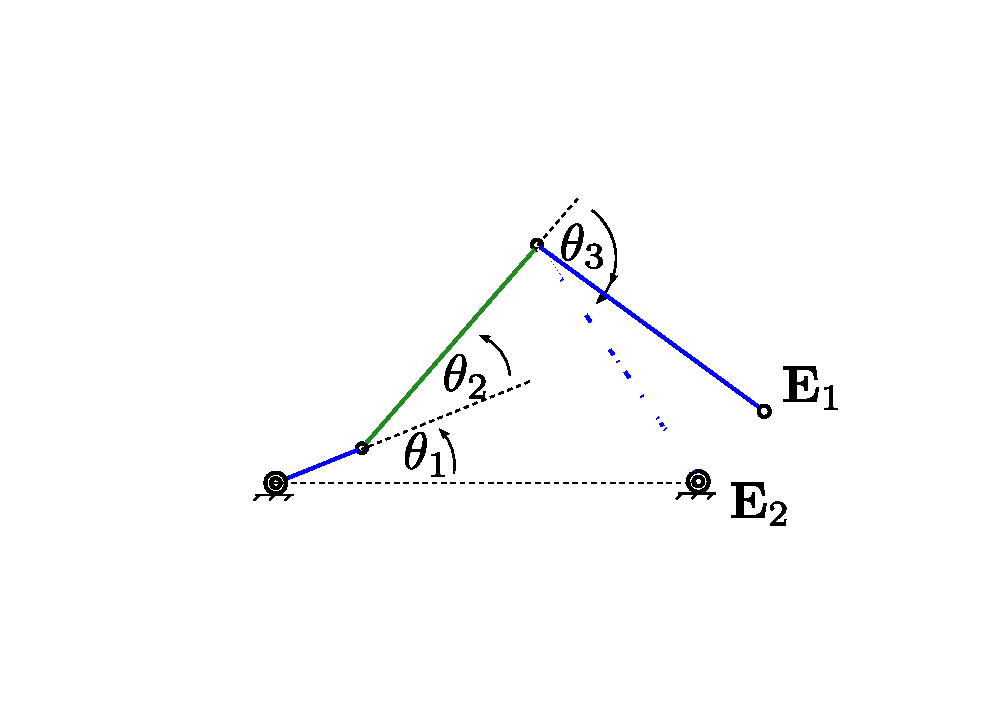
\includegraphics[width=100mm]{viergelenk.pdf}
		\caption{Structure of the Four-Bar Linkage. \\ \footnotesize{Source: Knoll, Carsten/ private illustration}}
	\end{figure}


	%%%%%%%%%%%%%%%%%%%%%% MDOEL EQUATIONS %%%%%%%%%%%%%%%%%%%%%%%%%%%

	\section{Model Equations} % MUST

	DAE Variables and Input Vector:
	\begin{align*}
		\underline{x} &= (p_1 \ p_2 \ q_1 \ \dot{p}_1 \ \dot{p}_2 \ \dot{q}_1 \ \lambda_1 \ \lambda_2)^T &= (x_1 \ x_2 \ x_3 \ \dot{x}_1 \ \dot{x}_2 \ \dot{x}_3 \ \lambda_1 \ \lambda_2)^T \\
		\underline{u} &= u_1
	\end{align*}

	\noindent Constraints:
	\begin{subequations}
	\begin{align}
		\l_1\cos(x_3) + l_2\cos(x_1 + x_3) - l_3\cos(x_2) - l_4 \\
		\l_1\sin(x_3) + l_2\sin(x_1 + x_3) - l_3\sin(x_2)
	\end{align}
	\end{subequations}

	\noindent System Equations:
	\begin{subequations}
	\begin{align*}
	0 &= J_2\ddot{x}_1 + J_2\ddot{x}_3 + g m_2 s_2\cos(x_1 + x_3) + l_1 m_2 \ddot{x}_3 s_2 \cos(x_1) + l_1 m_2 \dot{x}_3^2 s_2 \sin(x_1) \\
	&+ l_2 \lambda_1 \sin(x_1 + x_3) - l_2 \lambda_2 \cos(x_1 + x_3) + m_2 \ddot{x}_1 s_2^2 + m_2 \ddot{x}_3 s_2^2 \\
	\\
	0 &= J_3 \ddot{x}_2 + g m_3 s_3 \cos(x_2) - l_3 \lambda_1 \sin(x_2) + l_3 \lambda_2 \cos(x_2) + m_3 \ddot{x}_2 s_3^2 \\
	\\
	0 &= J_1 \ddot{x}_3 + J_2 \ddot{x}_1 + J_2 \ddot{x}_3 + g l_1 m_2 \cos(x_3) + g m_1 s_1 \cos(x_3) + g m_2 s_2 \cos(x_1 + x_3) \\
	&+ l_1^2 m_2 \ddot{x}_3 + l_1 \lambda_1 \sin(x_3) - l_1 \lambda_2 \cos(x_3) + l_1 m_2 \ddot{x}_1 s_2 \cos(x_1)- l_1 m_2 \dot{x}_1^2 s_2 \sin(x_1) \\
	&- 2 l_1 m_2 \dot{x}_1 \dot{x}_3 s_2 \sin(x_1) + 2 l_1 m_2 \ddot{x}_3 s_2 \cos(x_1)+ l_2 \lambda_1 \sin(x_1 + x_3) - l2 \lambda_2 \cos(x_1 + x_3) \\
	&+ m_1 \ddot{x}_3 s_1^2 + m_2 \ddot{x}_1 s_2^2 + m_2 \ddot{x}_3 s_2^2 - u_1 \\
	\end{align*}
	\end{subequations}

	%%%%%%%%%%%%%%%%%%%%%% PARAMETERS | OUTPUTS %%%%%%%%%%%%%%%%%%%%%%%%%%%
	\noindent
	Parameters: $s_1, \, s_2, \, s_3, \, m_1, \, m_2, \, m_3, \, J_1, \, J_2, \, J_3, \, l_1, \, l_2, \, l_3, \, l_4, \, g$% variables with constant, predefined value
	\\
	Outputs: $y, \, \dot{y}$ % MAY

	%%%%%%%%%%%%%%%%%%%%%% ASSUMPTIONS %%%%%%%%%%%%%%%%%%%%%%%%%%%


	%%%%%%%%%%%%%%%%%%%%%% EXEMPLARY PARAMETER VALUES %%%%%%%%%%%%%%%%%%%%%%%%%%%

	\subsection{Exemplary parameter values}
	\begin{tabular}{cl}
\hline
  Symbol  & Value                                                                                                                                                                                \\
\hline
   $A$    & $\left[\begin{matrix}0.8189 & 0.0863 & 0.09 & 0.0813\\0.2524 & 1.0033 & 0.0313 & 0.2004\\-0.0545 & 0.0102 & 0.7901 & -0.258\\-0.1918 & -0.1034 & 0.1602 & 0.8604\end{matrix}\right]$ \\
   $B$    & $\left[\begin{matrix}0.0045 & 0.0044\\0.1001 & 0.01\\0.0003 & -0.0136\\-0.0051 & 0.0936\end{matrix}\right]$                                                                          \\
 $B_{1}$  & $\left[\begin{matrix}0.0045 & 0.0044\\0.1001 & 0.01\\0.0003 & -0.0136\\-0.0051 & 0.0936\end{matrix}\right]$                                                                          \\
 $C_{1}$  & $\left[\begin{matrix}1.0 & 0 & -1.0 & 0\\0 & 0 & 0 & 0\\0 & 0 & 0 & 0\end{matrix}\right]$                                                                                            \\
   $C$    & $\left[\begin{matrix}1.0 & 0 & 0 & 0\\0 & 0 & 1.0 & 0\end{matrix}\right]$                                                                                                            \\
 $D_{11}$ & $\left[\begin{matrix}0 & 0 & 0\\0 & 0 & 0\\0 & 0 & 0\end{matrix}\right]$                                                                                                             \\
 $D_{12}$ & $\left[\begin{matrix}0 & 0\\1.0 & 0\\0 & 1.0\end{matrix}\right]$                                                                                                                     \\
 $D_{21}$ & $\left[\begin{matrix}0 & 1.0 & 0\\0 & 0 & 1.0\end{matrix}\right]$                                                                                                                    \\
\hline
\end{tabular}

	%%%%%%%%%%%%%%%%%%%%%% DERIVATION & EXPLANATION %%%%%%%%%%%%%%%%%%%%%%%%%%%

	\section{Derivation and Explanation} % SHOULD
	The Lagrangian mechanics was used for the solution.

	%%%%%%%%%%%%%%%%%%%%%% REFERENCES %%%%%%%%%%%%%%%%%%%%%%%%%%%

	\begin{thebibliography}{10}
		\bibitem{But21}Knoll, Carsten:
		\textit{Considered model: four-bar linkage (= two link manipulator + one link manipulator + rigid coupling)}, Jupyter Notebook published 2019. \\
		\url{https://github.com/TUD-RST/symbtools/blob/main/docs/demo_notebooks/modeltools/four-bar_linkage_model_and_simulation.ipynb}
	\end{thebibliography}

\end{document}

